\documentclass{article}

\usepackage{arxiv}

\usepackage[utf8]{inputenc} % allow utf-8 input
\usepackage[T1]{fontenc}    % use 8-bit T1 fonts
\usepackage{lmodern}        % https://github.com/rstudio/rticles/issues/343
\usepackage{hyperref}       % hyperlinks
\usepackage{url}            % simple URL typesetting
\usepackage{booktabs}       % professional-quality tables
\usepackage{amsfonts}       % blackboard math symbols
\usepackage{nicefrac}       % compact symbols for 1/2, etc.
\usepackage{microtype}      % microtypography
\usepackage{lipsum}
\usepackage{graphicx}

\title{Making the Most of BLUPS : \linebreak A Method for Estimating
Nonlinear Selection \linebreak on Behavioral Reaction Norms}

\author{
    Jordan S. Martin
   \\
    Human Ecology Group, Institute of Evolutionary Medicine \\
    University of Zurich \\
   \\
  \texttt{\href{mailto:jordan.martin@uzh.ch}{\nolinkurl{jordan.martin@uzh.ch}}} \\
  }

\usepackage{color}
\usepackage{fancyvrb}
\newcommand{\VerbBar}{|}
\newcommand{\VERB}{\Verb[commandchars=\\\{\}]}
\DefineVerbatimEnvironment{Highlighting}{Verbatim}{commandchars=\\\{\}}
% Add ',fontsize=\small' for more characters per line
\usepackage{framed}
\definecolor{shadecolor}{RGB}{248,248,248}
\newenvironment{Shaded}{\begin{snugshade}}{\end{snugshade}}
\newcommand{\AlertTok}[1]{\textcolor[rgb]{0.94,0.16,0.16}{#1}}
\newcommand{\AnnotationTok}[1]{\textcolor[rgb]{0.56,0.35,0.01}{\textbf{\textit{#1}}}}
\newcommand{\AttributeTok}[1]{\textcolor[rgb]{0.77,0.63,0.00}{#1}}
\newcommand{\BaseNTok}[1]{\textcolor[rgb]{0.00,0.00,0.81}{#1}}
\newcommand{\BuiltInTok}[1]{#1}
\newcommand{\CharTok}[1]{\textcolor[rgb]{0.31,0.60,0.02}{#1}}
\newcommand{\CommentTok}[1]{\textcolor[rgb]{0.56,0.35,0.01}{\textit{#1}}}
\newcommand{\CommentVarTok}[1]{\textcolor[rgb]{0.56,0.35,0.01}{\textbf{\textit{#1}}}}
\newcommand{\ConstantTok}[1]{\textcolor[rgb]{0.00,0.00,0.00}{#1}}
\newcommand{\ControlFlowTok}[1]{\textcolor[rgb]{0.13,0.29,0.53}{\textbf{#1}}}
\newcommand{\DataTypeTok}[1]{\textcolor[rgb]{0.13,0.29,0.53}{#1}}
\newcommand{\DecValTok}[1]{\textcolor[rgb]{0.00,0.00,0.81}{#1}}
\newcommand{\DocumentationTok}[1]{\textcolor[rgb]{0.56,0.35,0.01}{\textbf{\textit{#1}}}}
\newcommand{\ErrorTok}[1]{\textcolor[rgb]{0.64,0.00,0.00}{\textbf{#1}}}
\newcommand{\ExtensionTok}[1]{#1}
\newcommand{\FloatTok}[1]{\textcolor[rgb]{0.00,0.00,0.81}{#1}}
\newcommand{\FunctionTok}[1]{\textcolor[rgb]{0.00,0.00,0.00}{#1}}
\newcommand{\ImportTok}[1]{#1}
\newcommand{\InformationTok}[1]{\textcolor[rgb]{0.56,0.35,0.01}{\textbf{\textit{#1}}}}
\newcommand{\KeywordTok}[1]{\textcolor[rgb]{0.13,0.29,0.53}{\textbf{#1}}}
\newcommand{\NormalTok}[1]{#1}
\newcommand{\OperatorTok}[1]{\textcolor[rgb]{0.81,0.36,0.00}{\textbf{#1}}}
\newcommand{\OtherTok}[1]{\textcolor[rgb]{0.56,0.35,0.01}{#1}}
\newcommand{\PreprocessorTok}[1]{\textcolor[rgb]{0.56,0.35,0.01}{\textit{#1}}}
\newcommand{\RegionMarkerTok}[1]{#1}
\newcommand{\SpecialCharTok}[1]{\textcolor[rgb]{0.00,0.00,0.00}{#1}}
\newcommand{\SpecialStringTok}[1]{\textcolor[rgb]{0.31,0.60,0.02}{#1}}
\newcommand{\StringTok}[1]{\textcolor[rgb]{0.31,0.60,0.02}{#1}}
\newcommand{\VariableTok}[1]{\textcolor[rgb]{0.00,0.00,0.00}{#1}}
\newcommand{\VerbatimStringTok}[1]{\textcolor[rgb]{0.31,0.60,0.02}{#1}}
\newcommand{\WarningTok}[1]{\textcolor[rgb]{0.56,0.35,0.01}{\textbf{\textit{#1}}}}

% Pandoc citation processing
\newlength{\csllabelwidth}
\setlength{\csllabelwidth}{3em}
\newlength{\cslhangindent}
\setlength{\cslhangindent}{1.5em}
% for Pandoc 2.8 to 2.10.1
\newenvironment{cslreferences}%
  {}%
  {\par}
% For Pandoc 2.11+
\newenvironment{CSLReferences}[3] % #1 hanging-ident, #2 entry spacing
 {% don't indent paragraphs
  \setlength{\parindent}{0pt}
  % turn on hanging indent if param 1 is 1
  \ifodd #1 \everypar{\setlength{\hangindent}{\cslhangindent}}\ignorespaces\fi
  % set entry spacing
  \ifnum #2 > 0
  \setlength{\parskip}{#2\baselineskip}
  \fi
 }%
 {}
\usepackage{calc} % for calculating minipage widths
\newcommand{\CSLBlock}[1]{#1\hfill\break}
\newcommand{\CSLLeftMargin}[1]{\parbox[t]{\csllabelwidth}{#1}}
\newcommand{\CSLRightInline}[1]{\parbox[t]{\linewidth - \csllabelwidth}{#1}}
\newcommand{\CSLIndent}[1]{\hspace{\cslhangindent}#1}

\usepackage{amsmath, xparse, mathtools, upgreek}
\usepackage{lineno}
\linenumbers
\usepackage{hyperref}
\hypersetup{ colorlinks=true, linkcolor=black, citecolor=black, filecolor=black, urlcolor=black}


\begin{document}
\maketitle

\def\tightlist{}


\begin{abstract}
Individuals' behavioral strategies are often well described by reaction
norms, which are functions predicting repeatable patterns of phenotypic
consistency, plasticity, and predictability across an environmental
gradient. Reaction norms can be readily estimated using mixed-effects
models and play a key role in current theories of adaptive individual
variation. Unfortunately, however, it remains challenging to assess the
directional effects of reaction norms on fitness-relevant outcomes, due
to the high degree of uncertainty in random effect estimates of reaction
norm parameters, also known as best linear unbiased predictors (BLUPs).
Previous solutions to this problem avoid inferential bias by limiting
analyses to the description of linear covariances and correlations among
BLUPs and other measures. As such, empiricists currently lack a method
for exploring and explaining reaction norms effects with non-linear
structure, such as stabilizing, disruptive, or correlational selection,
which are crucial for testing adaptive theory of individual variation.
To address this issue, a solution is presented for unbiased estimation
of nonlinear reaction norm effects on fitness or any other outcome of
interest. This solution involves specifying BLUPs as both random and
fixed effects in a single Bayesian multi-response model. By
simultaneously accounting for uncertainty in BLUPs and their causal
effects on other traits, the risks accompanying classical approaches can
be effectively avoided. A novel method for visualizing multivariate
selection with such models is also proposed. Simulations are then used
to assess the power of these models under realistic empirical scenarios.
Coding tutorials are provided to aid researchers in applying these
models to their own datasets using R.
\end{abstract}

\keywords{
    mixed-effects
   \and
    multivariate
   \and
    Bayesian
   \and
    personality
   \and
    plasticity
   \and
    predictability
  }

\hypertarget{introduction}{%
\section{Introduction}\label{introduction}}

A population will evolve by natural selection whenever heritable
variation occurs in fitness-relevant phenotypes
(\protect\hyperlink{ref-Darwin}{Darwin 1859}). Individual differences in
behavior are, therefore, a fundamental ingredient of adaptive behavioral
evolution. Across taxa, repeatable individual variation is observed not
only in average behavior (\protect\hyperlink{ref-Bell2009}{Bell,
Hankison, and Laskowski 2009}), but also in the degree of behavioral
responsiveness exhibited toward the environment
(\protect\hyperlink{ref-Ding2010}{Dingemanse et al. 2010};
\protect\hyperlink{ref-Stamps2016}{Stamps 2016}), as well as in the
intra-individual variability of behavior across time
(\protect\hyperlink{ref-Biro2013}{Biro and Adriaenssens 2013};
\protect\hyperlink{ref-Westneat2015}{Westneat, Wright, and Dingemanse
2015}). These patterns of personality, plasticity, and predictability
represent distinct but often integrated components of organisms'
reaction norms (see \textbf{Figure \ref{fig:fig1}}), which are functions
expressing individual-specific behavioral strategies across
environmental gradients (\protect\hyperlink{ref-Ding2010}{Dingemanse et
al. 2010}; \protect\hyperlink{ref-McNamara2020}{McNamara and Leimar
2020}). The evolution of such function-valued traits is currently a
central area of research within evolutionary ecology
(\protect\hyperlink{ref-Gomulk2018}{Gomulkiewicz et al. 2018}), which
has led to a host of methodological innovations for estimating the RNs
of labile phenotypes subject to measurement error
(\protect\hyperlink{ref-DingDocht2013}{Dingemanse and Dochtermann 2013};
\protect\hyperlink{ref-Martin2021}{Martin and Jaeggi 2021}), as well as
the development of a rich theoretical framework for explaining the
adaptive processes maintaining individual variation in RNs within
populations (\protect\hyperlink{ref-Dall2014}{Dall and Griffith 2014};
\protect\hyperlink{ref-Sih2015}{Sih et al. 2015};
\protect\hyperlink{ref-Wolf2010}{Wolf and Weissing 2010}).

For labile phenotypes such as behavior, hormones, and cognition, the
magnitude of repeatable between-individual variation is generally modest
in comparison to the total phenotypic variation observed across space
and time (\protect\hyperlink{ref-Bell2009}{Bell, Hankison, and Laskowski
2009}; \protect\hyperlink{ref-Cauch2018}{Cauchoix et al. 2018};
\protect\hyperlink{ref-Fanson2019}{Fanson and Biro 2015}). This is
unsurprising, given that these traits are often the primary mechanisms
by which organisms can flexibly respond to ephemeral and stochastic
variation in their local environments, such as by up-regulating
circulating testosterone in response to social challenges
(\protect\hyperlink{ref-Eis2011}{Eisenegger, Haushofer, and Fehr 2011}),
or by temporarily inducing a fear state in response to odor cues of
predation (\protect\hyperlink{ref-Mathuru2012}{Mathuru et al. 2012}). As
such, single measurements of these labile phenotypes are poor indicators
of the underlying between-individual differences that are targeted by
selection, and tend to instead reflect various sources of
within-individual environmental heterogeneity
(\protect\hyperlink{ref-Brommer2013}{Brommer 2013};
\protect\hyperlink{ref-DingDocht2013}{Dingemanse and Dochtermann 2013}).
Despite the unfortunate fact that many empirical studies still confound
these distinct sources of trait (co)variation
(\protect\hyperlink{ref-Niem2018}{Niemelä and Dingemase 2018};
\protect\hyperlink{ref-Roy2018}{Royauté et al. 2018}), the necessity of
longitudinal data for studying RNs is increasingly appreciated and
enforced within behavioral ecology
(\protect\hyperlink{ref-Ding2020}{Dingemanse and Wright 2020}). With the
appropriate application of generalized mixed-effect models (GLMMs),
these repeated measures data can then be used to estimate the unobserved
but statistically identifiable RNs underlying raw behavioral
measurements, thus effectively partitioning stochastic effects and
measurement error from repeatable sources of individual variation
(\protect\hyperlink{ref-DingDocht2013}{Dingemanse and Dochtermann 2013};
\protect\hyperlink{ref-Martin2021}{Martin and Jaeggi 2021};
\protect\hyperlink{ref-Naka2010}{Nakagawa and Schielzeth 2010};
\protect\hyperlink{ref-Nus2007}{Nussey, Wilson, and Brommer 2007}).

GLMMs are a powerful tool for not only estimating RNs from empirical
data using random effects, but also for subsequently modeling the fixed
effects of personality, plasticity, and predictability on fitness and
the expression of other phenotypes. Nevertheless, although GLMMs are
quite robust (\protect\hyperlink{ref-Schiel2020}{Schielzeth et al.
2020}), they can only give as much information about RNs and their
effects as the model assumptions and empirical data provided to them.
For labile phenotypes like behavior, this means that the predicted
random effect values of RN parameters, also known as best linear
unbiased predictors (BLUPs), are often estimated with non-trivial
degrees of statistical uncertainty. The use of BLUP point estimates to
predict outcomes in another response model will, therefore, artificially
reduce uncertainty in the estimated effects of RNs and increase the risk
of false positives (see \protect\hyperlink{ref-Hadfield2010}{Hadfield et
al. 2010} for a detailed treatment, \textbf{Figure \ref{fig:fig1}}).
Previous solutions to this problem have provided effective antidotes to
the anti-conservative inference encouraged by ignoring uncertainty in
BLUPs (\protect\hyperlink{ref-Hous2017}{Houslay and Wilson 2017}), but
this comes at the cost of a reduced capacity to effectively model
complex, directional effects of RNs on fitness-relevant outcomes and
other phenotypes (see \textbf{Figure \ref{fig:fig2}}). Therefore, the
present study introduces a novel Bayesian multivariate modelling
approach to facilitate unbiased estimation of RN effects of arbitrary
complexity. The proposed solution is first motivated through a brief
discussion of \protect\hyperlink{ref-Hous2017}{Houslay and Wilson}
(\protect\hyperlink{ref-Hous2017}{2017}) 's approach to the misuse of
BLUPs and its benefits and limitations, as well as introduction to
Bayesian inference for unfamiliar readers. Novel Bayesian models are
then introduced conceptually and demonstrated in multiple simulated
empirical scenarios based on prior research. Code for estimating these
models with the Stan statistical programming language
(\protect\hyperlink{ref-Stan}{Carpenter et al. 2017}) in the R
statistical environment (\protect\hyperlink{ref-Rbase}{R Core Team
2020}) is also provided to aid researchers in unbiasedly modeling RN
effects in their own datasets (see electronic supplementary material
{[}\textbf{ESM}{]}).

\begin{figure}
  \centering
  \fbox{\rule[-.5cm]{8cm}{11cm} \rule[-.5cm]{8cm}{0cm}}
  \caption{Sample figure caption.}
  \label{fig:fig1}
\end{figure}

\hypertarget{the-current-solution}{%
\section{The current solution}\label{the-current-solution}}

The basic challenge of modelling RN effects is to effectively account
for the uncertainty in RN parameters (i.e.~BLUPs) across all stages of
analysis. Variation in phenotypes with low to moderate repeatability is,
by definition, largely explained by factors other than
between-individual differences. As a consequence, sampling designs with
modest repeated measurements and uncontrolled environmental variation
typically result in highly uncertain estimation of RNs. Failure to
account for the uncertainty of RNs across subsequent stages of analysis
artificially reduces uncertainty in the inferred effects of RNs, as
uncertainty in individuals' trait values necessarily translates into
uncertainty about the effects of these trait values. This is
demonstrated in \textbf{Figure \ref{fig:fig1}}, where it can be seen
that the probability of false positives remains undesirably high for
BLUP point estimates even when using conservative Bayesian priors. For
this reason, \protect\hyperlink{ref-Hadfield2010}{Hadfield et al.}
(\protect\hyperlink{ref-Hadfield2010}{2010}) discouraged all future use
of BLUP point estimates in evolutionary ecology, so as to prevent the
proliferation of misleading findings in the literature. Nevertheless,
because the theoretical significance of RNs is not diminished by the
difficulty of appropriately modeling their effects, many behavioral
ecologists without clear alternative solutions continued to misuse point
estimates of BLUPs in their research. In response,
\protect\hyperlink{ref-Hous2017}{Houslay and Wilson}
(\protect\hyperlink{ref-Hous2017}{2017}) provided a detailed overview of
appropriate strategies for tackling this challenge, emphasizing that
multivariate GLMMs with correlated random effects can be used to
effectively account for uncertainty in RNs across multiple response
models. Despite these repeated cautionary notes, some researchers still
continue to utilize BLUP point estimates (e.g.
\protect\hyperlink{ref-Ding2020b}{Dingemanse et al. 2020}) or raw data
(e.g. \protect\hyperlink{ref-Brehm2019}{Brehm et al. 2019}) for testing
RN effects, even while acknowledging the work of
\protect\hyperlink{ref-Hadfield2010}{Hadfield et al.}
(\protect\hyperlink{ref-Hadfield2010}{2010}) and
\protect\hyperlink{ref-Hous2017}{Houslay and Wilson}
(\protect\hyperlink{ref-Hous2017}{2017}). This likely reflects the fact
that the random effects models proposed by
\protect\hyperlink{ref-Hous2017}{Houslay and Wilson}
(\protect\hyperlink{ref-Hous2017}{2017}) do not readily extend to a
variety of more complex RN effects that cannot be straightforwardly
derived from random effect covariances and correlations (see
\textbf{Figure \ref{fig:fig2}}). This section briefly reviews the
proposed solution of \protect\hyperlink{ref-Hous2017}{Houslay and
Wilson} (\protect\hyperlink{ref-Hous2017}{2017}) for the misuse of BLUPs
and discusses its benefits and limitations.

\hypertarget{multivariate-glmms-with-covarying-random-effects}{%
\subsection{Multivariate GLMMs with covarying random
effects}\label{multivariate-glmms-with-covarying-random-effects}}

\protect\hyperlink{ref-Hous2017}{Houslay and Wilson}
(\protect\hyperlink{ref-Hous2017}{2017}) note that many behavioral
ecologists rely on GLMM software packages such as lme4
(\protect\hyperlink{ref-Bates2014}{Bates et al. 2014}) that do not
readily address multivariate, integrated phenotypes. As a consequence,
researchers are often motivated to (i) estimate RNs from a univariate
response model of the relevant behavior, and (ii) subsequently enter
BLUP point estimates of these RNs as covariates in another response
model. Fortunately, the risk engendered by this approach can be readily
overcome by specifying a multivariate GLMM that simultaneously accounts
for uncertainty in behavioral BLUPs and their associations with other
responses. \protect\hyperlink{ref-Hous2017}{Houslay and Wilson}
(\protect\hyperlink{ref-Hous2017}{2017}) demonstrate how this can be
done with random effect correlations for phenotypic and quantitative
genetic studies using both frequentist and Bayesian software. For
simplicity, the present study focuses on the estimation of phenotypic
GLMMs, although it should be noted that these models can be
straightforwardly extended to quantitative genetic animal models (see
\textbf{ESM}); further note that the present study relies on the
flexibility of Bayesian modelling software for the novel solutions
proposed below, and classical estimators are thus not considered
further. Researchers unfamiliar with the general benefits of fully
Bayesian inference are encouraged to see
\protect\hyperlink{ref-Rethinking}{McElreath}
(\protect\hyperlink{ref-Rethinking}{2020}) for detailed discussion, as
well as \protect\hyperlink{ref-Gelman2020}{Gelman et al.}
(\protect\hyperlink{ref-Gelman2020}{2020}) for helpful tips on
developing an effective Bayesian workflow for data analysis.

Consider a situation where we are interested to know whether
personality, plasticity, and predictability are associated across
phenotypes \(y\) and \(z\). Plasticity is considered across some
environmental gradient \(x\), and we assume for simplicity that
environmental exposures are randomized across individuals, so that there
is no need to within-individual center the covariate (van de
\protect\hyperlink{ref-Pol2009}{Pol and Wright 2009}). A bivariate GLMM
can be specified to estimate the associations among these RN parameters
from repeated measures data. In particular, for observation \emph{i} of
individual \emph{j}. \begin{align} \tag{1.1}\label{eq:1.1}
y_{ij} & \sim f \left(\eta^{(y)}_{ij }, \theta^{(y)}_{j} \right) \\
z_{ij} & \sim f \left( \eta^{(z)}_{ij}, \theta^{(z)}_{j} \right) \nonumber \\
g^{(y)} \left( \eta^{(y)}_{ij} \right) &= \mu_j^{(y)}+\beta_j^{(y)}x_{ij} \nonumber \\
g^{(z)} \left( \eta^{(z)}_{ij} \right) &= \mu_j^{(z)}+\beta_j^{(z)}x_{ij} \nonumber \\
\begin{bmatrix}
\boldsymbol{\mu}^{(y)} &
\boldsymbol{\beta}^{(y)} &
\boldsymbol{\theta}^{(y)} & 
...  &
\boldsymbol{\theta}^{(z)}
\end{bmatrix} ^\textrm{T}
 \sim \mathrm{M}&\mathrm{VNormal} \left(
\begin{bmatrix}
{\mu^{(y)}_0} &
{\beta^{(y)}_1} &
{\theta^{(y)}_0} &
... &
{\theta^{(z)}_0}
\end{bmatrix}^\textrm{T},\boldsymbol{\mathrm{P}} \right) \nonumber
\end{align}

Bold values are used to distinguish vectors and matrices from scalars,
and superscripts \((y)\) and \((z)\) are used to distinguish parameters
specific to the respective response models. The traits values are
specified as being generated by some probability density function \(f\)
with corresponding location \(\boldsymbol{\eta}\) and dispersion
\(\boldsymbol{\theta}\) parameters, e.g.~the means and standard
deviations of a normal distribution or the means and shape parameters of
gamma, negative binomial, and beta distributions. For GLMMs, these
parameters are modelled on a latent linear scale using a link function
\(g\) (e.g.~an identity, log, logistic, or reciprocal transformation).
We therefore refer to \(g(\eta_{ij})\) as the linear predictor for
observation \emph{i} of individual \emph{j}.

Typically, personality and plasticity are modelled through the linear
predictor of the location parameters \(\boldsymbol{\eta}\), capturing
variation in expected behavior (i.e.~predicted behavior averaged over
dispersion). This is accomplished through the estimation of random
intercept \(\mu_j\) and random slope \(\beta_j\) for individual \(j\),
corresponding to the elevation and slope of the individual's behavioral
RN. Predictability is instead modelled through the RN dispersion
parameters \(\boldsymbol{\theta}\), which are also random effects
capturing individual-specific variability independent of the linear
predictor. For simplicity, we ignore the possibility that individuals
may also exhibit plasticity in their predictability as a function of the
environment, although this could be readily estimated (along with other
fixed and random effects) by introducing an additional linear predictor
\(g(\theta_{ij})\). For distributions without an explicit dispersion
parameter, such as Poisson or binomial distributions, individual
differences in predictability cannot be directly modelled in this way,
but they can nonetheless be derived using the assumed mean-variance
relations of these distributions (see \textbf{ESM} for example models
handling both scenarios).

The individual-specific random effects are generated from a multivariate
normal distribution centered on the population-average intercepts
(\(\mu_0\)), slopes (\(\beta_1\)), and dispersion parameters
(\(\theta_0\)) for each trait. The answer to our inquiry of
interest--how do personality, plasticity, and predictability associate
across traits \(y\) and \(z\)--is thus found in the covariance matrix
\(\boldsymbol{\mathrm{P}}\) for the RN parameters.
\begin{align} \tag{1.2}\label{eq:1.2}
\boldsymbol{\mathrm{P}} & =
\begin{pmatrix}
\mathrm{var} ( \boldsymbol{\mu}^{(y)} ) & 
\mathrm{cov} (\boldsymbol{\mu}^{(y)}, \boldsymbol{\beta}^{(y)} ) &
...  & \mathrm{cov} (\boldsymbol{\mu}^{(y)}, \boldsymbol{\theta}^{(z)} ) \\
\mathrm{cov} ( \boldsymbol{\beta}^{(y)}, \boldsymbol{\mu}^{(y)} ) & \mathrm{var} ( \boldsymbol{\beta}^{(y)} ) &
... & \mathrm{cov} (\boldsymbol{\beta}^{(y)}, \boldsymbol{\theta}^{(z)} ) \\
\vdots & \vdots & \ddots & \vdots \\
\mathrm{cov} (\boldsymbol{\theta}^{(z)}, \boldsymbol{\mu}^{(y)} ) &
\mathrm{cov} (\boldsymbol{\theta}^{(z)}, \boldsymbol{\beta}^{(y)} ) &
\cdots &  \mathrm{var} ( \boldsymbol{\theta}^{(z)} )
\end{pmatrix}
\end{align}

In many cases, researchers will lack sufficient data to confidently
estimate these parameters, and will instead consider simpler models such
as models with only covarying personality components
\(\mathrm{cov} (\boldsymbol{\mu}^{(y)}, \boldsymbol{\mu}^{(z)} )\).
\protect\hyperlink{ref-Hous2017}{Houslay and Wilson}
(\protect\hyperlink{ref-Hous2017}{2017}) also provide further
considerations for modelling linear selection effects without repeated
fitness measures. It is nevertheless important to recognize the full
potential of such an analysis for capturing the structure of RNs and
behavioral syndromes, which is further integrate into the novel models
presented below.

\hypertarget{fully-bayesian-inference}{%
\subsection{Fully Bayesian inference}\label{fully-bayesian-inference}}

To estimate this model within a Bayesian framework, we simply need to
specify prior distributions for all the population-level parameters,
which are transformed within the model to derive the individual-level RN
parameters. \begin{align} \tag{1.3}\label{eq:1.3}
\mu_0^{(y)},\beta_1^{(y)},...,\sigma_0^{(z)},\boldsymbol{\mathrm{P}} \sim \boldsymbol{f}(\boldsymbol{\Phi})
\end{align}

As above, \(\boldsymbol{f}\) are probability density functions for each
parameter and \(\boldsymbol{\Phi}\) are the corresponding distributional
parameters. Although it is common for methods papers to use and/or
recommend using highly diffuse or flat priors (e.g.
\protect\hyperlink{ref-Hous2017}{Houslay and Wilson 2017};
\protect\hyperlink{ref-Vill2016}{Villemereuil et al. 2016}), it is also
well established within the statistics literature that weakly
informative, regularizing priors--which pool hypotheses toward null
values and provide low probability to extreme effect sizes--facilitate
more robust inferences and should generally be preferred over flat
priors whenever possible (\protect\hyperlink{ref-Gelman2000}{Gelman and
Tuerlinckx 2000}; \protect\hyperlink{ref-Rethinking}{McElreath 2020};
\protect\hyperlink{ref-Lemoine2019}{Lemoine 2019}). This does not
require that one has access to a relevant meta-analysis or is in a
position to make strong a priori assumptions about the true effect size
(cf. \protect\hyperlink{ref-Ellison2004}{Ellison 2004}). Rather, one can
simply use general-purpose, conservative priors as a means of increasing
the generalizability and robustness of their findings, even in a state
of relative ignorance about the true effect size. See
\protect\hyperlink{ref-Lemoine2019}{Lemoine}
(\protect\hyperlink{ref-Lemoine2019}{2019}) for a more detailed
discussion and recommendations for weakly regularizing priors in
ecological research, which are described further in the \textbf{ESM}.

By specifying priors in the model, all parameters will be subsequently
estimated as posterior distributions. For example, individual \emph{j}'s
RN parameters on trait \(y\) will no longer be estimated with BLUP point
estimates \(\hat{\mu}_j^{(y)}\), \(\hat{\beta}_j^{(y)}\), and
\(\hat{\theta}_j^{(y)}\), but will instead be estimated as probability
distributions capturing all of the statistical uncertainty in the BLUPs
\begin{align} \tag{2.1}\label{eq:2.1}
\mathrm{Pr}\left( \mu_j^{(y)} \ | \ \boldsymbol{x},\boldsymbol{y},\boldsymbol{z},...,\boldsymbol{\Phi} \right), \quad
\mathrm{Pr}\left( \beta_j^{(y)} \ | \ \boldsymbol{x},\boldsymbol{y},\boldsymbol{z},...,\boldsymbol{\Phi} \right), \quad
\mathrm{Pr}\left( \theta_j^{(y)} \ | \ \boldsymbol{x},\boldsymbol{y},\boldsymbol{z},...,\boldsymbol{\Phi} \right)
\end{align}

The answer to the question ``What are the estimated BLUPs for individual
\emph{j}'s RN parameters?'' is now given as series of probability
distributions, capturing all uncertainty in these values conditional on
the observed dataset (\(\boldsymbol{x},\boldsymbol{y},\boldsymbol{z}\))
and other model parameters and priors (\(...\Phi\)). Given that all
uncertainty is captured in these distributions, the model provides
nearly unlimited flexibility for direct forms of hypothesis testing. For
example, to quantify our confidence that there is more repeatable
variation in personality than predictability for trait \(y\), we simply
need to manipulate the relevant posteriors to calculate
\begin{align} \tag{2.2}\label{eq:2.2}
\mathrm{Pr}\left( \mathrm{var} ( \boldsymbol{\mu}^{(y)} )  > \mathrm{var} ( \boldsymbol{\theta}^{(y)} )  \ \mid \ \boldsymbol{x},\boldsymbol{y},\boldsymbol{z},...,\boldsymbol{\Phi} \right)
\end{align}

When posterior distributions are estimated with Markov Chain Monte Carlo
(MCMC), this value can be easily quantified by simply assessing this
inequality across the relevant vectors of posterior samples and
calculating the proportion of samples for which it is satisfied (see
\textbf{SEM} for examples). Note that this is \emph{not} an indirect
null hypothesis test, which gives the probability of observing the data
under the assumption that the null hypothesis is true. Instead, it is a
direct test of a biologically substantive hypothesis given the observed
data, the evaluation of which is generally the primary goal of
scientific research. As such, intuitive interpretation can be made of
this posterior probability, so that values closer to 1 indicate greater
support for this directional hypothesis and values closer to 0 indicate
stronger support for the opposite directional hypothesis. One could
similarly perform a direct hypothesis test of a more robust null
hypothesis than is typically considered, not merely quantifying the
probability that the effect size is exactly zero, which is almost never
true in reality (\protect\hyperlink{ref-Amrhein2019}{Amrhein, Trafimow,
and Greenland 2019}; \protect\hyperlink{ref-Meehl1978}{Meehl 1978};
\protect\hyperlink{ref-Gelman2017}{Gelman and Carlin 2017}), but rather
the probability that the effect is of a biologically trivial magnitude
(e.g.~\textless{} \textbar0.1\textbar). For instance, considering the
population-average regression coefficient for trait \(z\)
\begin{align} \tag{2.3}\label{eq:2.3}
\mathrm{Pr}\left( -0.1 < \beta_1^{(z)}  < 0.1  \ \mid \ \boldsymbol{x},\boldsymbol{y},\boldsymbol{z},...,\boldsymbol{\Phi} \right)
\end{align}

These Bayesian hypothesis tests help empiricists to avoid many common
misinterpretations of classical tests, such as interpreting confidence
intervals as reflecting the probable range of the true effect,
interpreting \emph{P}-values as providing the probability of the null
hypothesis being true, or interpreting the rejection of a null
hypothesis test as being indicative of the true (``alternative'')
hypothesis being correct (\protect\hyperlink{ref-Green2016}{Greenland et
al. 2016}; \protect\hyperlink{ref-Rethinking}{McElreath 2020};
\protect\hyperlink{ref-McShane2019}{McShane et al. 2019}). Furthermore,
as should be obvious from these examples, Bayesian posteriors can be
easily manipulated to address a variety of questions which may not be
easily specified directly in a statistical model. This provides
theoretically important benefits such as being able to perform
hypothesis tests with random effects (e.g.~comparisons of specific plot,
group, or individual differences) or any other quantity that can be
derived from the initial model parameters {[}e.g.~comparisons of
repeatabilities or \(R^2\) values, or tests of the magnitude of
assortment coefficients and social selection differentials;
\protect\hyperlink{ref-Martin2021}{Martin and Jaeggi}
(\protect\hyperlink{ref-Martin2021}{2021}){]}.

\hypertarget{benefits-and-limitations}{%
\subsection{Benefits and limitations}\label{benefits-and-limitations}}

As should be clear, the multivariate GLMMs proposed by
\protect\hyperlink{ref-Hous2017}{Houslay and Wilson}
(\protect\hyperlink{ref-Hous2017}{2017}) are an extremely valuable tool
for behavioral ecologists interested in RNs, integrated phenotypes, and
adaptive individual variation. When estimated within a Bayesian
framework, these models provide a great deal of flexibility for
addressing a variety of questions beyond simply quantifying random
effect variances and covariances, although this on its own is quite an
important task. As any student of multivariate statistics is well aware,
trait covariance matrices such as \(\boldsymbol{\mathrm{P}}\) can be
readily transformed to provide a veritable treasure chest of biological
insights (\protect\hyperlink{ref-Blows2007}{Blows 2007}), such as
identifying trajectories of phenotypic conservation and divergence among
closely related populations (\protect\hyperlink{ref-Roy2020}{Royauté,
Hedrick, and Dochtermann 2020}), discovering latent behavioral
characters and networks causing covariance among multiple traits
(\protect\hyperlink{ref-Araya2014}{Araya-Ajoy and Dingemanse 2014};
\protect\hyperlink{ref-Martin2019}{Martin et al. 2019}), and calculating
selection differentials and genetic responses to selection
(\protect\hyperlink{ref-Stinch2014}{Stinchcombe, Simonsen, and Blows
2014}). Thus, with the flexible hypothesis testing provided by Bayesian
inference, \protect\hyperlink{ref-Hous2017}{Houslay and Wilson}
(\protect\hyperlink{ref-Hous2017}{2017}) 's method can be used to
accomplish many important empirical goals with relative ease.

Nonetheless, there are important cases where further information is
desired that cannot be straightforwardly derived from random effect
covariances alone, which places limitations on the flexibility of this
method for exploring and explaining the causal effects of RNs on
evolutionarily relevant outcomes. These considerations are not specific
to the models proposed by \protect\hyperlink{ref-Hous2017}{Houslay and
Wilson} (\protect\hyperlink{ref-Hous2017}{2017}), but are general
limitations of all purely variance-partitioning models, which achieve
accurate predictions and characterizations of (co)variance at the
potential cost of reduced explanatory power and insight about the causal
interactions generating (co)variances
(\protect\hyperlink{ref-Briley2019}{Briley et al. 2019};
\protect\hyperlink{ref-Hadfield2017}{Hadfield and Thomson 2017};
\protect\hyperlink{ref-Okasha2020}{Okasha and Otsuka 2020}). This is why
fixed effects remain important for testing evolutionary ecological
theory, because we often want to directly parameterize specific
functional relationships between traits, as well as to specify the
direction of these effects. In other words, we often want to know
whether trait \(y\) affects \(z\) in a specific, potentially non-linear
manner, and perhaps in interaction with other traits or states, rather
than merely asking whether trait \(y\) and \(z\) are linearly associated
through any number of possible causal pathways in either direction.

In particular, testing adaptive theory of individual variation often
requires evaluating nonlinear selection on behavioral RNs
(\textbf{Figure \ref{fig:fig2}}), which can be approximated using
quadratic and interaction effects on RN parameters in a parametric
fitness model (\protect\hyperlink{ref-Lande1983}{Lande and Arnold
1983}). If the population RN is at an evolutionary equilibrium, soc that
RN variation is non-adaptive within the population and results from
processes such as mutation-selection balance or developmental noise
(e.g. \protect\hyperlink{ref-Bierbach2017}{Bierbach, Laskowski, and Wolf
2017}; \protect\hyperlink{ref-Tooby1990}{Tooby and Cosmides 1990}), then
we should expect to find evidence of stabilizing selection around the
population average RN parameters. This would be observed in a
Lande-Arnold selection analysis on independent RN parameters as null or
weak linear effects and negative quadratic effects
(\protect\hyperlink{ref-Stinch2008}{Stinchcombe et al. 2008}).
Alternatively, strong disruptive selection, potentially indicative of an
ongoing behaviorally-mediated speciation process
(\protect\hyperlink{ref-Wolf2012}{Wolf and Weissing 2012}), would be
expected to surface as the opposite pattern--i.e.~null or weak linear
effects with positive quadratic effects. In other situations, such as
when variation in RNs is maintained through spatially and/or temporally
varying selection (e.g. \protect\hyperlink{ref-Gurven2014}{Gurven et al.
2014}; Le \protect\hyperlink{ref-LC2015}{Cœur et al. 2015}), interaction
effects will also be expected between local ecological conditions
(e.g.~population density, resource abundance, climate) and individuals'
RN parameters across multiple selection events. Similar considerations
apply to social contexts as considered by evolutionary game theory, in
which frequency-dependent fitness functions, such as cooperative
strategies with diminishing returns or threshold payoffs as a function
of partners' strategies (\protect\hyperlink{ref-McNamara2020}{McNamara
and Leimar 2020}), will be observed through interactive selection
effects (\protect\hyperlink{ref-Araya2020}{Araya-Ajoy, Westneat, and
Wright 2020}; \protect\hyperlink{ref-Martin2021}{Martin and Jaeggi
2021}; \protect\hyperlink{ref-Queller2011}{Queller 2011}). When
considering behavioral syndromes, RNs may also be expected to evolve
through correlational selection for specific parameter combinations,
such as through female mate choice of males with high levels of both
personality and predictability in aggressiveness among cichlids
(\emph{Pelvicachromis pulcher},
\protect\hyperlink{ref-Scherer2018}{Scherer, Kuhnhardt, and Schuett
2018}). When RN parameters are under correlational selection, trait
interaction effects will be observed in a selection analysis,
irrespective of the linear main effects of each trait
(\protect\hyperlink{ref-Blows2003}{Blows 2003}). Of course, these
considerations also apply to a host of other RN effects on outcomes
other than fitness, such as the exponential effects of personality in
activity level and anxiety on seed removal and dispersal distance,
respectively, among small mammals in the northeastern United States
(\protect\hyperlink{ref-Brehm2019}{Brehm et al. 2019}). In all such
cases, one could not detect these theoretically pertinent relationships
using random effect covariances alone, because covariance is by
definition a measure of linear dependency and thus does not capture
non-linear dependencies among traits.

It should be noted that one apparent but flawed solution to these
challenges is to (i) first estimate BLUP posteriors in an initial
Bayesian random effects model, and then to (ii) estimate a separate
model with RN effects estimated by running the analysis repeatedly over
every MCMC sample of the BLUP posteriors. While this is technically
carrying the uncertainty in RNs forward, it nonetheless is expected to
result in downwardly biased estimates of the RN effects, as
\protect\hyperlink{ref-Ding2020}{Dingemanse and Wright}
(\protect\hyperlink{ref-Ding2020}{2020}) observed in supplementary
simulations. Although these authors do not provide an explanation for
the observed bias, it can be attributed to a more general statistical
phenomena known as attenuation bias, in which independent measurement
error in a predictor variable causes downward bias in its association
with an outcome measure (\protect\hyperlink{ref-Adolf2007}{Adolph and
Hardin 2007}; \protect\hyperlink{ref-Spearman1904}{Spearman 1904}). This
is caused by the fact that the BLUPs in the initial model are estimated
independently of the RN effects on the outcome of interest, so that the
estimated uncertainty in BLUPs is by design statistically independent of
uncertainty in the RN effect estimated in the second stage of the
analysis. This does not, however, make the use of BLUP point estimates
any less dangerous, but is instead simply an artifact of not
simultaneously accounting for both sources of uncertainty in the same
model. It is important to remember that BLUPs are latent, statistical
inferences, not directly measured trait values or mere averages of raw
trait values, and as such are particularly sensitive to correct model
specification (\protect\hyperlink{ref-Hadfield2010}{Hadfield et al.
2010}; \protect\hyperlink{ref-Postma2006}{Postma 2006}).

\hypertarget{a-novel-solution}{%
\section{A novel solution}\label{a-novel-solution}}

Given the limitations of relying solely on covarying random effects,
behavioral ecologists stand to benefit from adding an additional
modeling approach to their toolkit, one capable of directly estimating
nonlinear RN effects of arbitrary complexity. Here I propose a novel
solution that is a straightforward extension of
\protect\hyperlink{ref-Hous2017}{Houslay and Wilson}
(\protect\hyperlink{ref-Hous2017}{2017}) `s previous work: Bayesian
multi-response GLMMs in which individuals' RNs are simultaneously
treated as random effects on their observed behaviors as well as fixed
effects on outcome measures of interest (e.g.~survival and reproduction,
habitat choice, performance in an experimental task, etc.). In this
section, this basic modelling approach is formally introduced, along
with various extensions of interest for specific empirical scenarios. A
novel and straightforward method for visualizing the within-generation
effects of multivariate selection is also proposed to compliment models
considering selection on more than two RN parameters. Simulations are
then used to explore the statistical properties of these models under
realistic sampling regimes, providing a guidepost for researchers
interested in applying these models to their own datasets. Finally, to
aid in this effort, detailed R coding tutorials are provided in the
\textbf{ESM}.

\hypertarget{multivariate-glmms-for-nonlinear-selection-on-rns}{%
\subsection{Multivariate GLMMs for nonlinear selection on
RNs}\label{multivariate-glmms-for-nonlinear-selection-on-rns}}

Our goal in overcoming the limitations of previous approaches is to
specify a multi-response GLMM for observation \(i\) of individual \(j\)
on repeatedly measured behavior \(y\), as well as for fitness-relevant
outcome \(w\) predicted by individual variation in RN parameters of
\(y\). Given that researchers will often lack repeated measures of
fitness or fitness-proxies (e.g.~survival, clutch size, mate choice),
the presented models assume that a single fitness measure is available
per individual, although they can be straightforwardly extended for
repeated measures by including additional random effects. It is also
important to note that, to the best knowledge of the author, none of
these models can be estimated with mainstream statistical software. This
does not, however, reflect any fundamental issue with their
parameterization or interpretation, but rather pragmatic limitations of
the estimators employed and/or the software syntax. The Stan statistical
programming language (\protect\hyperlink{ref-Stan}{Carpenter et al.
2017}), which relies on cutting-edge and computationally efficient MCMC
algorithms, provides exceptional flexibility for specifying and
straightforwardly estimating such atypical GLMMs within a Bayesian
framework.

\hypertarget{gaussian-fitness-measures}{%
\subsubsection{Gaussian fitness
measures}\label{gaussian-fitness-measures}}

For simplicity, we begin by assuming that the fitness measure can be
effectively modelled with a Gaussian distribution, which simplifies the
estimation of selection gradients and differentials. As is appropriate
for modelling relative fitness (\protect\hyperlink{ref-Lande1983}{Lande
and Arnold 1983}), \(w\) is mean-scaled so that \(w_j = W_j/\bar{W}\),
prior to entering the analysis. Our basic approach will be to specify
the model of phenotype \(y\) as described in \textbf{Eq \ref{eq:1.1}}.
However, we need to change how the random effects are centered in the
model, because we'd like for the individual RN trait values to be
centered on zero in the fitness model. To accomplish this, we specify an
alternative but equivalent non-centered parameterization, in which the
scale of the population-average parameters is separated out from the
specification of the individual-specific parameters. This makes it so
that the BLUPs are estimated are centered on zero and expressed as
deviations from the population average. To accomplish this for the
dispersion parameter, we also need to introduce an additional linear
predictor \(g^{(y)} \left( \theta^{(y)}_{ij} \right)\) to account for
nonlinearity on the original scale due to adding parameters on the
transformed linear scale.

\begin{equation} \tag{3.1}\label{eq:3.1}
\begin{gathered}[t]
y_{ij} \sim f \left(\eta^{(y)}_{ij }, \theta^{(y)}_{ij} \right)  \\
g_\eta \left( \eta^{(y)}_{ij} \right) = \mu_0^{(y)} + \mu_j^{(y)}+ \left(\beta_1 + \beta_j^{(y)} \right) x_{ij} \nonumber \\
g_\theta \left( \theta^{(y)}_{ij} \right) = \theta_0^{(y)} + \theta_{j}^{(y)} \nonumber \\
\begin{bmatrix}
\boldsymbol{\mu}^{(y)} &
\boldsymbol{\beta}^{(y)} &
\boldsymbol{\theta}^{(y)} \end{bmatrix} ^\textrm{T}
 \sim \mathrm{M}\mathrm{VNormal} \left(
\boldsymbol{0},\boldsymbol{\mathrm{P}} \right) \nonumber \\ \nonumber \\
w_{j} \sim \mathrm{Normal} \left( \mu _{j}, \upsigma _{j} \right) \nonumber \\
\mu _{j} = \mu _0 + \beta_1 \left( \mu^{(y)}_{j} \right) + 
                \beta_2 \left( \beta_j^{(y)} \right) + 
                \beta_3 \left( \theta^{(y)}_{j} \right) \\ 
                + \beta_4 \left( \mu^{(y)}_j \mu^{(y)}_j \right) +
                \beta_5\left( \beta^{(y)}_j \beta^{(y)}_j \right) +
                \beta_6 \left( \theta^{(y)}_j \theta^{(y)}_j \right)\\ 
                +  \beta_7 \left( \mu^{(y)}_j \beta^{(y)}_j \right) + 
                \beta_8 \left( \mu^{(y)}_j \theta^{(y)}_j \right) + 
                 \beta_9 \left( \beta^{(y)}_j \theta^{(y)}_j \right) \nonumber \\ 
\end{gathered}
\end{equation}

shorten to matrix notation\ldots{}

\hypertarget{within-generation-effects-of-selection}{%
\subsubsection{Within-generation effects of
selection}\label{within-generation-effects-of-selection}}

\ldots{}

\hypertarget{non-gaussian-fitness-measures}{%
\subsubsection{Non-Gaussian fitness
measures}\label{non-gaussian-fitness-measures}}

introduce \ldots{} approach of Morrissey \ldots{}

\hypertarget{visualizing-multivariate-selection}{%
\subsubsection{Visualizing multivariate
selection}\label{visualizing-multivariate-selection}}

issues with canonical analysis, PCA, \ldots{}

propose simple p

Fig 3\ldots{}

\hypertarget{simulation-of-model-properties}{%
\section{Simulation of model
properties}\label{simulation-of-model-properties}}

Table 1\ldots{}

\hypertarget{conclusion}{%
\section{Conclusion}\label{conclusion}}

\label{sec:others}

\lipsum[8] some text
(\protect\hyperlink{ref-kour2014real}{\textbf{kour2014real?}};
\protect\hyperlink{ref-kour2014fast}{\textbf{kour2014fast?}}) and see
(\protect\hyperlink{ref-hadash2018estimate}{\textbf{hadash2018estimate?}}).

The documentation for \verb+natbib+ may be found at

\begin{center}
  \url{http://mirrors.ctan.org/macros/latex/contrib/natbib/natnotes.pdf}
\end{center}

Of note is the command \verb+\citet+, which produces citations
appropriate for use in inline text. For example,

\begin{verbatim}
   \citet{hasselmo} investigated\dots
\end{verbatim}

produces

\begin{quote}
  Hasselmo, et al.\ (1995) investigated\dots
\end{quote}

\begin{center}
  \url{https://www.ctan.org/pkg/booktabs}
\end{center}

\hypertarget{figures}{%
\subsection{Figures}\label{figures}}

\lipsum[10] See Figure \ref{fig:fig1}. Here is how you add footnotes.
{[}\^{}Sample of the first footnote.{]}

\lipsum[11]

\begin{Shaded}
\begin{Highlighting}[]
\FunctionTok{plot}\NormalTok{(mtcars}\SpecialCharTok{$}\NormalTok{mpg)}
\end{Highlighting}
\end{Shaded}

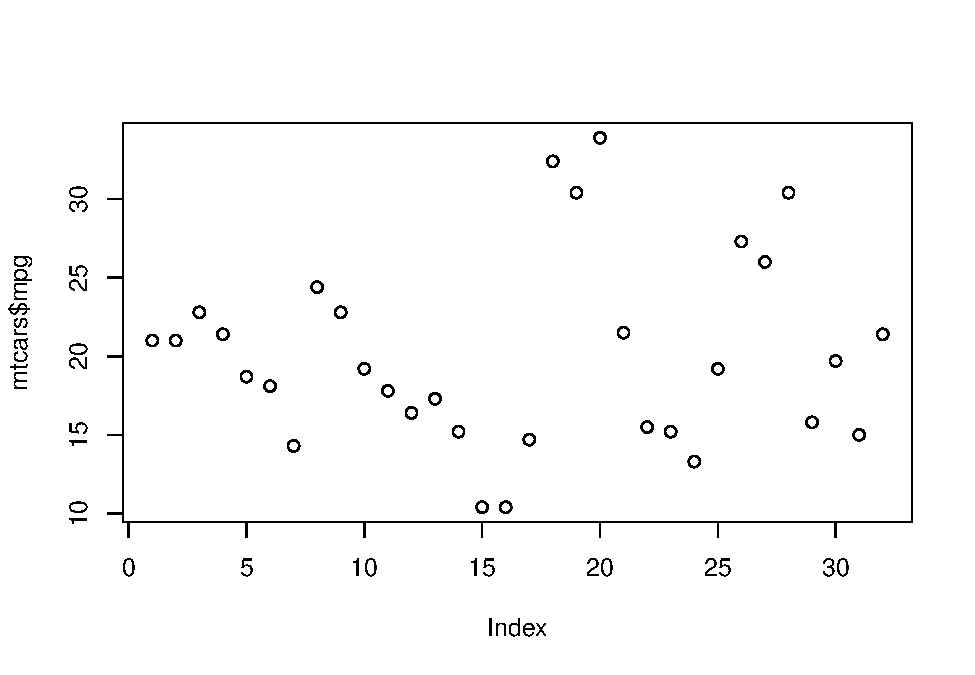
\includegraphics{BLUP-manuscript_files/figure-latex/unnamed-chunk-1-1.pdf}

\begin{figure}
  \centering
  \fbox{\rule[-.5cm]{4cm}{4cm} \rule[-.5cm]{4cm}{0cm}}
  \caption{Sample figure caption.}
  \label{fig:fig2}
\end{figure}

\hypertarget{tables}{%
\subsection{Tables}\label{tables}}

\lipsum[12]

See awesome Table\textasciitilde{}\ref{tab:table}.

\begin{table}
 \caption{Sample table title}
  \centering
  \begin{tabular}{lll}
    \toprule
    \multicolumn{2}{c}{Part}                   \\
    \cmidrule(r){1-2}
    Name     & Description     & Size ($\mu$m) \\
    \midrule
    Dendrite & Input terminal  & $\sim$100     \\
    Axon     & Output terminal & $\sim$10      \\
    Soma     & Cell body       & up to $10^6$  \\
    \bottomrule
  \end{tabular}
  \label{tab:table}
\end{table}

\hypertarget{lists}{%
\subsection{Lists}\label{lists}}

\begin{itemize}
\tightlist
\item
  Lorem ipsum dolor sit amet
\item
  consectetur adipiscing elit.
\item
  Aliquam dignissim blandit est, in dictum tortor gravida eget. In ac
  rutrum magna.
\end{itemize}

\hypertarget{leftovers}{%
\subsection{Leftovers}\label{leftovers}}

Previous To address this issue, empiricists have been encouraged to
forgo the use of BLUP point estimates as directional predictors
(i.e.~fixed effect covariates), and to instead estimate random effect
correlations (or covariances) among BLUPs and other relevant traits in a
multi-response model {[}\ldots{]}. This straightforward approach has
undoubtedly been important for reducing the risk of false positives
present in the literature, and is generally sufficient for empirical
studies in which researchers are content to describe the (partial)
correlations among traits. However, as with any purely
variance-partitioning model, this approach trades off explanatory
insight for descriptive accuracy {[}\ldots{]}. As a result, empiricists
currently lack a means of both avoiding bias due to the uncertainty in
BLUPs, as well as effectively identifying the potentially complex
directional effects of BLUPs on fitness and other phenotypes.

The present paper addresses this limitation by proposing an additional
modelling approach for the empiricist's toolkit: Bayesian multi-response
GLMMs with BLUPs specified as both random and fixed effects. This
approach is first motivated through a brief discussion of previously
proposed solutions and their limitations for identifying and explaining
some important behavioral phenomena. I then explain how fully Bayesian
multi-response models can be employed to avoid the misuse of BLUPs while
also modelling BLUP effects of arbitrary complexity. This demonstrated
through worked simulations of , with R code provided for estimating each

longitudinal datasets has GLMMs has increasingly become the norm within
evolutionary ecology. Despite the many benefits of GLMMs, inferential
bias has arisen in the literature from their application to causal
questions regarding directional effects of RN parameters.

However, despite the centrality of RNs to behavioral evolution, it
currently remains difficulty to unbiasedly investigate the causal
effects of RNs on fitness and the phenotypic expression of other traits.
Fundamentally, this is due to the high degree of , which is observed
across a host of behaviors in both wild and captive contexts. \ldots{}
While previous solutions have been provided for avoiding such
anti-conservative inference, these approaches are limited in their
capacity to address the complex, directional effects of RNs {[}see fig
2{]} .

\hypertarget{refs}{}
\begin{CSLReferences}{1}{0}
\leavevmode\hypertarget{ref-Adolf2007}{}%
Adolph, S. C., and J. S. Hardin. 2007. {``Estimating Phenotypic
Correlations: Correcting for Bias Due to Intraindividual Variability.''}
\emph{Functional Ecology} 21: 178--84.

\leavevmode\hypertarget{ref-Amrhein2019}{}%
Amrhein, V., D. Trafimow, and S. Greenland. 2019. {``Inferential
Statistics as Descriptive Statistics: There Is No Replication Crisis If
We Don't Expect Replication.''} \emph{The American Statistician} 73:
262--70.

\leavevmode\hypertarget{ref-Araya2014}{}%
Araya-Ajoy, Y. G., and N. J. Dingemanse. 2014. {``Characterizing
Behavioural {`Characters'}: An Evolutionary Framework.''}
\emph{Proceedings of the Royal Society B} 281: 20132645.

\leavevmode\hypertarget{ref-Araya2020}{}%
Araya-Ajoy, Y. G., D. F. Westneat, and J. Wright. 2020. {``Pathways to
Social Evolution and Their Evolutionary Feedbacks.''} \emph{Evolution}
74: 1894--1907.

\leavevmode\hypertarget{ref-Bates2014}{}%
Bates, D., M. Mächler, B. Bolker, and S. Walker. 2014. {``Fitting Linear
Mixed-Effects Models Using Lme4.''} \emph{arXiv Preprint} 1406.5823.

\leavevmode\hypertarget{ref-Bell2009}{}%
Bell, A. M., S. J. Hankison, and K. L. Laskowski. 2009. {``The
Repeatability of Behaviour: A Meta-Analysis.''} \emph{Animal Behaviour}
77: 771--83.

\leavevmode\hypertarget{ref-Bierbach2017}{}%
Bierbach, D., K. L. Laskowski, and M. Wolf. 2017. {``Behavioural
Individuality in Clonal Fish Arises Despite Near-Identical Rearing
Conditions.''} \emph{Nature Communications} 8: 1--7.

\leavevmode\hypertarget{ref-Biro2013}{}%
Biro, P. A., and B. Adriaenssens. 2013. {``Predictability as a
Personality Trait: Consistent Differences in Intraindividual Behavioral
Variation.''} \emph{The American Naturalist} 182: 621--29.

\leavevmode\hypertarget{ref-Blows2003}{}%
Blows, M. W. 2003. {``Measuring Nonlinear Selection.''} \emph{The
American Naturalist} 2003: 815--20.

\leavevmode\hypertarget{ref-Blows2007}{}%
---------. 2007. {``A Tale of Two Matrices: Multivariate Approaches in
Evolutionary Biology.''} \emph{Journal of Evolutionary Biology} 20:
1--8.

\leavevmode\hypertarget{ref-Brehm2019}{}%
Brehm, A. M., A. Mortelliti, G. A. Maynard, and J. Zydlewski. 2019.
{``Land‐use Change and the Ecological Consequences of Personality in
Small Mammal.''} \emph{Ecology Letters} 22: 1387--95.

\leavevmode\hypertarget{ref-Briley2019}{}%
Briley, D. A., J. Livengood, J. Derringer, E. M. Tucker-Drob, R. C.
Fraley, and B. W. Roberts. 2019. {``Interpreting Behavior Genetic
Models: Seven Developmental Processes to Understand.''} \emph{Behavioral
Genetics} 49: 196--210.

\leavevmode\hypertarget{ref-Brommer2013}{}%
Brommer, J. E. 2013. {``On Between-Individual and Residual (Co)
Variances in the Study of Animal Personality: Are You Willing to Take
the 'Individual Gambit'?''} \emph{Behavioral Ecology and Sociobiology}
67: 1027--32.

\leavevmode\hypertarget{ref-Stan}{}%
Carpenter, B., A. Gelman, M. D. Hoffman, D. Lee, B. Goodrich, M.
Betancourt, and... A. Riddell. 2017. {``Stan: A Probabilistic
Programming Language.''} \emph{Journal of Statistical Software} 74.
\url{https://www.jstatsoft.org/article/view/v076i01}.

\leavevmode\hypertarget{ref-Cauch2018}{}%
Cauchoix, M., P. K. Y. Chow, J. O. Van Horik, C. M. Atance, E. J.
Barbeau,...G. Barragan-Jason, and L. Cauchard. 2018. {``The
Repeatability of Cognitive Performance: A Meta-Analysis.''}
\emph{Philosophical Transactions of the Royal Society B} 373: 20170281.

\leavevmode\hypertarget{ref-LC2015}{}%
Cœur, C. C., M. Thibault, B. Pisanu, S. Thibault, J. L. Chapuis, and E.
Baudry. 2015. {``Temporally Fluctuating Selection on a Personality Trait
in a Wild Rodent Population.''} \emph{Behavioral Ecology} 26: 1285--91.

\leavevmode\hypertarget{ref-Dall2014}{}%
Dall, S. R. X., and S. C. Griffith. 2014. {``An Empiricist Guide to
Animal Personality Variation in Ecology and Evolution.''}
\emph{Frontiers in Ecology and Evolution} 14: 3.

\leavevmode\hypertarget{ref-Darwin}{}%
Darwin, C. 1859. \emph{On the Origin of Species by Means of Natural
Selection}. London, UK: J. Murray.

\leavevmode\hypertarget{ref-DingDocht2013}{}%
Dingemanse, N. J., and N. A. Dochtermann. 2013. {``Quantifying
Individual Variation in Behaviour: Mixed‐effect Modelling Approaches.''}
\emph{Journal of Animal Ecology} 82: 39--54.

\leavevmode\hypertarget{ref-Ding2010}{}%
Dingemanse, N. J., A. J. Kazem, D. Réale, and J. Wright. 2010.
{``Behavioural Reaction Norms: Animal Personality Meets Individual
Plasticity.''} \emph{Trends in Ecology and Evolution} 25: 81--89.

\leavevmode\hypertarget{ref-Ding2020b}{}%
Dingemanse, N. J., M. Moiron, Y. G. Araya‐Ajoy, A. Mouchet, and R. N.
Abbey‐Lee. 2020. {``Individual Variation in Age‐dependent Reproduction:
Fast Explorers Live Fast but Senesce Young?''} \emph{Journal of Animal
Ecology} 89: 601--13.

\leavevmode\hypertarget{ref-Ding2020}{}%
Dingemanse, N. J., and J. Wright. 2020. {``Criteria for Acceptable
Studies of Animal Personality and Behavioural Syndromes.''}
\emph{Ethology} 126: 865--69.

\leavevmode\hypertarget{ref-Eis2011}{}%
Eisenegger, C., J. Haushofer, and E. Fehr. 2011. {``The Role of
Testosterone in Social Interaction.''} \emph{Trends in Cognitive
Sciences} 15: 263--71.

\leavevmode\hypertarget{ref-Ellison2004}{}%
Ellison, A. M. 2004. {``Bayesian Inference in Ecology.''} \emph{Ecology
Letters} 7: 509--20.

\leavevmode\hypertarget{ref-Fanson2019}{}%
Fanson, K. V., and P. A. Biro. 2015. {``Meta-Analytic Insights into
Factors Influencing the Repeatability of Hormone Levels in Agricultural,
Ecological, and Medical Fields.''} \emph{American Journal of
Physiology-Regulatory, Integrative and Comparative Physiology} 316:
R101--9.

\leavevmode\hypertarget{ref-Gelman2017}{}%
Gelman, A., and J. Carlin. 2017. {``Some Natural Solutions to the
p-Value Communication Problem---and Why They Won't Work.''}
\emph{Journal of the American Statistician} 112: 899--901.

\leavevmode\hypertarget{ref-Gelman2000}{}%
Gelman, A., and F. Tuerlinckx. 2000. {``Type s Error Rates for Classical
and Bayesian Single and Multiple Comparison Procedures.''}
\emph{Computational Statistics} 15: 373--90.

\leavevmode\hypertarget{ref-Gelman2020}{}%
Gelman, A., A. Vehtari, D. Simpson, C. C. Margossian, B. Carpenter, Y.
Yao, and... M. Modrák. 2020. {``Bayesian Workflow.''} \emph{arXiv
Preprint} arXiv:2011.01808. \url{https://arxiv.org/abs/2011.01808}.

\leavevmode\hypertarget{ref-Gomulk2018}{}%
Gomulkiewicz, R., J. G. Kingsolver, P. A. Carter, and N. Heckman. 2018.
{``Variation and Evolution of Function-Valued Traits.''} \emph{Annual
Review of Ecology, Evolution, and Systematics} 49: 139--64.

\leavevmode\hypertarget{ref-Green2016}{}%
Greenland, S., S. J. Senn, K. J. Rothman, J. B. Carlin, C. Poole, S. N.
Goodman, and D. G. Altman. 2016. {``Statistical Tests, p Values,
Confidence Intervals, and Power: A Guide to Misinterpretations.''}
\emph{European Journal of Epidemiology} 31: 337--50.

\leavevmode\hypertarget{ref-Gurven2014}{}%
Gurven, M., C. von Rueden, J. Stieglitz, H. Kaplan, and D. E. Rodriguez.
2014. {``The Evolutionary Fitness of Personality Traits in a Small-Scale
Subsistence Society.''} \emph{Evolution and Human Behavior} 35: 17--25.

\leavevmode\hypertarget{ref-Hadfield2017}{}%
Hadfield, J. D., and C. E. Thomson. 2017. {``Interpreting Selection When
Individuals Interact.''} \emph{Methods in Ecology and Evolution} 8:
688--99.

\leavevmode\hypertarget{ref-Hadfield2010}{}%
Hadfield, J. D., A. J. Wilson, D. Garant, and B. C. Sheldon. 2010.
{``The Misuse of BLUP in Ecology and Evolution.''} \emph{The American
Naturalist} 175: 116--25.

\leavevmode\hypertarget{ref-Hous2017}{}%
Houslay, T. M., and A. J. Wilson. 2017. {``Avoiding the Misuse of BLUP
in Behavioural Ecology.''} \emph{Behavioral Ecology} 28: 948--52.

\leavevmode\hypertarget{ref-Lande1983}{}%
Lande, R., and S. J. Arnold. 1983. {``The Measurement of Selection on
Correlated Characters.''} \emph{Evolution} 37: 1210--26.

\leavevmode\hypertarget{ref-Lemoine2019}{}%
Lemoine, N. P. 2019. {``Moving Beyond Noninformative Priors: Why and How
to Choose Weakly Informative Priors in Bayesian Analyses.''}
\emph{Oikos} 128.
\url{https://onlinelibrary.wiley.com/doi/full/10.1111/oik.05985}.

\leavevmode\hypertarget{ref-Martin2021}{}%
Martin, J. S., and A. V. Jaeggi. 2021. {``Social Animal Models for
Quantifying Plasticity, Assortment, and Selection on Interacting
Phenotypes.''} \emph{Journal of Evolutionary Biology} XX: XX--.

\leavevmode\hypertarget{ref-Martin2019}{}%
Martin, J. S., J. J. Massen, V. Šlipogor, T. Bugnyar, A. V. Jaeggi, and
S. E. Koski. 2019. {``The EGA+ GNM Framework: An Integrative Approach to
Modelling Behavioural Syndromes.''} \emph{Methods in Ecology and
Evolution} 10: 245--57.

\leavevmode\hypertarget{ref-Mathuru2012}{}%
Mathuru, A. S., C. Kibat, W. F. Cheong, G. Shui, M. R. Wenk, R. W.
Friedrich, and S. Jesuthasan. 2012. {``Chondroitin Fragments Are
Odorants That Trigger Fear Behavior in Ffsh.''} \emph{Current Biology}
22: 538--54.

\leavevmode\hypertarget{ref-Rethinking}{}%
McElreath, R. 2020. \emph{Statistical Rethinking: A Bayesian Course with
Examples in r and Stan}. 2nd ed. CRC Press.
\url{https://xcelab.net/rm/statistical-rethinking/}.

\leavevmode\hypertarget{ref-McNamara2020}{}%
McNamara, J. M., and O. Leimar. 2020. \emph{Game Theory in Biology}.
Oxford, UK: Oxford University Press.

\leavevmode\hypertarget{ref-McShane2019}{}%
McShane, B. B., D. Gal, A. Gelman, C. Robert, and J. L. Tackett. 2019.
{``Abandon Statistical Significance.''} \emph{The American Naturalist}
73: 235--45.

\leavevmode\hypertarget{ref-Meehl1978}{}%
Meehl, P. E. 1978. {``Theoretical Risks and Tabular Asterisks: Sir Karl,
Sir Ronald, and the Slow Progress of Soft Psychology.''} \emph{Journal
of Consulting and Clinical Psychology} 46: 806--34.

\leavevmode\hypertarget{ref-Naka2010}{}%
Nakagawa, S., and H. Schielzeth. 2010. {``Repeatability for Gaussian and
Non‐gaussian Data: A Practical Guide for Biologists.''} \emph{Biological
Reviews} 85: 935--56.

\leavevmode\hypertarget{ref-Niem2018}{}%
Niemelä, P. T., and N. J. Dingemase. 2018. {``Meta-Analysis Reveals Weak
Associations Between Intrinsic State and Personality.''}
\emph{Proceedings of the Royal Society B} 285: 20172823.

\leavevmode\hypertarget{ref-Nus2007}{}%
Nussey, D. H., A. J. Wilson, and J. E. Brommer. 2007. {``The
Evolutionary Ecology of Individual Phenotypic Plasticity in Wild
Populations.''} \emph{Journal of Evolutionary Biology} 20: 831--44.

\leavevmode\hypertarget{ref-Okasha2020}{}%
Okasha, S., and J. Otsuka. 2020. {``The Price Equation and the Causal
Analysis of Evolutionary Change.''} \emph{Philosophical Transactions of
the Royal Society B} 375: 20190365.

\leavevmode\hypertarget{ref-Pol2009}{}%
Pol, M. van de, and J. Wright. 2009. {``A Simple Method for
Distinguishing Within- Versus Between-Subject Effects Using Mixed
Models.''} \emph{Animal Behaviour} 77: 753--58.

\leavevmode\hypertarget{ref-Postma2006}{}%
Postma, E. 2006. {``Implications of the Difference Between True and
Predicted Breeding Values for the Study of Natural Selection and
Micro‐evolution.''} \emph{Journal of Evolutionary Biology} 19: 309--20.

\leavevmode\hypertarget{ref-Queller2011}{}%
Queller, D. C. 2011. {``Expanded Social Fitness and Hamilton's Rule for
Kin, Kith, and Kind.''} \emph{Proceedings of the National Academy of
Sciences USA} 108: 10792--99.

\leavevmode\hypertarget{ref-Rbase}{}%
R Core Team. 2020. \emph{R: A Language and Environment for Statistical
Computing}. Vienna, Austria: R Foundation for Statistical Computing.
\url{https://www.R-project.org}.

\leavevmode\hypertarget{ref-Roy2018}{}%
Royauté, R., M. A. Berdal, C. R. Garrison, and N. A. Dochtermann. 2018.
{``A Meta-Analysis of the Pace-of-Life Syndrome Hypothesis.''}
\emph{Behavioral Ecology and Sociobiology} 72: 1--10.

\leavevmode\hypertarget{ref-Roy2020}{}%
Royauté, R., A. Hedrick, and N. A. Dochtermann. 2020. {``Behavioural
Syndromes Shape Evolutionary Trajectories via Conserved Genetic
Architecture.''} \emph{Proceedings of the Royal Society B} 287:
20200183.

\leavevmode\hypertarget{ref-Scherer2018}{}%
Scherer, U., M. Kuhnhardt, and W. Schuett. 2018. {``Predictability Is
Attractive: Female Preference for Behaviourally Consistent Males but No
Preference for the Level of Male Aggression in a Bi-Parental Cichlid.''}
\emph{PloS One} 13: e0195766.

\leavevmode\hypertarget{ref-Schiel2020}{}%
Schielzeth, H., N. J. Dingemanse, S. Nakagawa, D. F. Westneat, H.
Allegue, C. Teplitsky, and Y. G. Araya-Ajoy. 2020. {``Robustness of
Linear Mixed Effects Models to Violations of Distributional
Assumptions.''} \emph{Methods in Ecology and Evolution} 11: 1141--52.

\leavevmode\hypertarget{ref-Sih2015}{}%
Sih, A., K. J. Mathot, M. Moirón, P. O. Montiglio, M. Wolf, and N. J.
Dingemanse. 2015. {``Animal Personality and State--Behaviour Feedbacks:
A Review and Guide for Empiricists.''} \emph{Trends in Ecology and
Evolution} 30: 50--60.

\leavevmode\hypertarget{ref-Spearman1904}{}%
Spearman, C. 1904. {``The Proof and Measurement of Association Between
Two Things.''} \emph{The American Journal of Psychology} 15: 72--101.

\leavevmode\hypertarget{ref-Stamps2016}{}%
Stamps, J. A. 2016. {``Individual Differences in Behavioural
Plasticities.''} \emph{Biological Reviews} 91: 534--67.

\leavevmode\hypertarget{ref-Stinch2008}{}%
Stinchcombe, J. R., A. F. Agrawal, P. A. Hohenlohe, S. J. Arnold, and M.
W. Blows. 2008. {``Estimating Nonlinear Selection Gradients Using
Quadratic Regression Coefficients: Double or Nothing?''}
\emph{Evolution} 68.
\url{https://onlinelibrary.wiley.com/doi/full/10.1111/evo.12321}.

\leavevmode\hypertarget{ref-Stinch2014}{}%
Stinchcombe, J. R., A. K. Simonsen, and M. W. Blows. 2014. {``Estimating
Uncertainty in Multivariate Responses to Selection.''} \emph{Evolution}
68. \url{https://onlinelibrary.wiley.com/doi/full/10.1111/evo.12321}.

\leavevmode\hypertarget{ref-Tooby1990}{}%
Tooby, J., and L. Cosmides. 1990. {``On the Universality of Human Nature
and the Uniqueness of the Individual: The Role of Genetics and
Adaptation.''} \emph{Journal of Personality} 58: 17--67.

\leavevmode\hypertarget{ref-Vill2016}{}%
Villemereuil, P. de, H. Schielzeth, S. Nakagawa, and M. Morrissey. 2016.
{``General Methods for Evolutionary Quantitative Genetic Inference from
Generalized Mixed Models.''} \emph{Genetics} 204: 1281--94.

\leavevmode\hypertarget{ref-Westneat2015}{}%
Westneat, D. F., J. Wright, and N. J. Dingemanse. 2015. {``The Biology
Hidden Inside Residual Within‐individual Phenotypic Variation.''}
\emph{Biological Reviews} 90: 729--43.

\leavevmode\hypertarget{ref-Wolf2010}{}%
Wolf, M., and F. J. Weissing. 2010. {``An Explanatory Framework for
Adaptive Personality Differences.''} \emph{Philosophical Transactions of
the Royal Society B} 365: 3959--68.

\leavevmode\hypertarget{ref-Wolf2012}{}%
---------. 2012. {``Animal Personalities: Consequences for Ecology and
Evolution.''} \emph{Trends in Ecology \& Evolution} 27: 452--61.

\end{CSLReferences}

\bibliographystyle{unsrt}
\bibliography{mybibfile.bib}


\end{document}
